%%%%%%%%%%%%%%%%%%%%%%%%%%%%%%%%%%%%%%%%%%%%%%%%%%%%%%%%%%%%%%%%%%%%%%%%%%%%%%%%

\documentclass[a4paper, 10pt ]{article}     

% The following packages can be found on http:\\www.ctan.org
\usepackage{graphics} % for pdf, bitmapped graphics files
\usepackage{epsfig} % for postscript graphics files
\usepackage{mathptmx} % assumes new font selection scheme installed
\usepackage{times} % assumes new font selection scheme installed
\usepackage{amsmath} % assumes amsmath package installed
\usepackage{amssymb}  % assumes amsmath package installed
\usepackage[usenames]{color}
\usepackage[utf8]{inputenc} 

\title{\LARGE \bf
 Pré-manip Handibio
}


\author{Claire Dune, Cyril Joly}



\begin{document}
\maketitle
\thispagestyle{empty}
\pagestyle{empty}
%%%%%%%%%%%%%%%%%%%%%%%%%%%%%%%%%%%%%%%%%%%%%%%%%%%%%%%%%%%%%%%%%%%%%%%%%%%%%%%%

\section{Objectif de l'expérimentation}

L'objectif de cette expérimentation est triple : 
\begin{enumerate}
\item aquérir la posture lors de la marche avec et sans déambulateur pour pouvoir établir des comparaisons. 
\item aquérir des informations avec le déambulateur instrumenté.
\item prendre en main tous les systèmes d'acquisition pour les futures manips
\end{enumerate}

\section{Protocole}

Chaque sujet devra parcourir 5m en avant, en marchant tout droit. Sur ces 5m, au moins 3 m devraient être complétement couverts par la zone de travail des caméras. Les conditions expérimentales suivantes seront testées 5 fois pour chaque personnes : 

\begin{enumerate}
\item Marche sans déambulateur à allure normale.
\item Marche sans déambulateur à allure lente en trainant les pieds.
\item Marche avec déambulateur en s'appuyant sur le déambulateur a allure normale.
\item Marche avec déambulateur en s'appuyant sur le déambulateur et en trainant des pieds.
\end{enumerate}

\section{Matériel}

Dans cette manip, nous utiliserons les 6 caméras Qualysis ainsi qu'un déambulateur équipé de capteurs.

\subsection{Utilisation du Qualisys}

Pour cette expérience, il faut positionner les caméras de sorte à avoir une zone étalonnée qui couvre un chemin rectiligne de 3m de long permettant de voir à la fois les pieds et la tête du marcheur. \\

\subsection{Utilisation du logiciel}
Voici la marche à suivre pour utiliser le soft Qualisys.

\begin{enumerate}
\item positionner les 6 caméras approximativement pour couvrir la zone de travail
\item Brancher les caméras sur le secteur + les cables USB et ethernet
\item Configuration du réseau : Qualisys DHCP serveur (attention, réseau local à IP fixe)
\item Lancer le soft Qualisys track manager (indication 120Hz maxi)
\item Réglages $>$ Caméra $>$ Connection pour localiser les 6 caméras. Lorsque les 6 caméras sont localisées, on peut changer la fréquence d'acquisition. Pour la calibration, il faut une minute a 200 Hz, soit 12 000 frames.
\item File $>$ new ... pour créer la nouvelle manip
\item Calibration
\begin{enumerate}
\item fixer la duree de la calibration a une minute au moins pour une grande zone de travail.
\item lancer la calibration
\item pour que le résultat soit bon, il faut un résidu $r<1$
\item une fois la calibration faite, on peut afficher la zone calibrée pour vérifier la précision sur la zone de travail.
\end{enumerate}
\item Enregistrer la manip
\item Labéliser (touche MAJ+L)
\item On peut ensuite faire une création de modèle pour pouvoir le réutiliser pour les autres manips. (touche MAJ + B). Le menu s'appelle "AIM Generate Model"
\end{enumerate}


\subsubsection{Positionnement des marqueurs sur le sujet }

La figure \ref{fig:definitionQ} présente un modèle géométrique simplifié de l'homme avec les différents degrès de liberté de ses articulations.
Les figures \ref{fig:marqueursFace} et \ref{fig:marqueursDos} présentent  un positionnement des marqueurs respectivement sur une vue de face  et sur une vue de dos du sujet. Pour positionner les marqueurs, on se base sur les recommandation de la société international de biomécanique \cite{Wu02, Wu05}.
\begin{figure}
\includegraphics[width=0.7\columnwidth]{images/modeleHommeQ.eps}
\label{fig:definitionQ}
\caption{Représentation géométrique simplifiée du corps humain pour identifier les degrès de liberté.}
\end{figure}

\begin{figure}
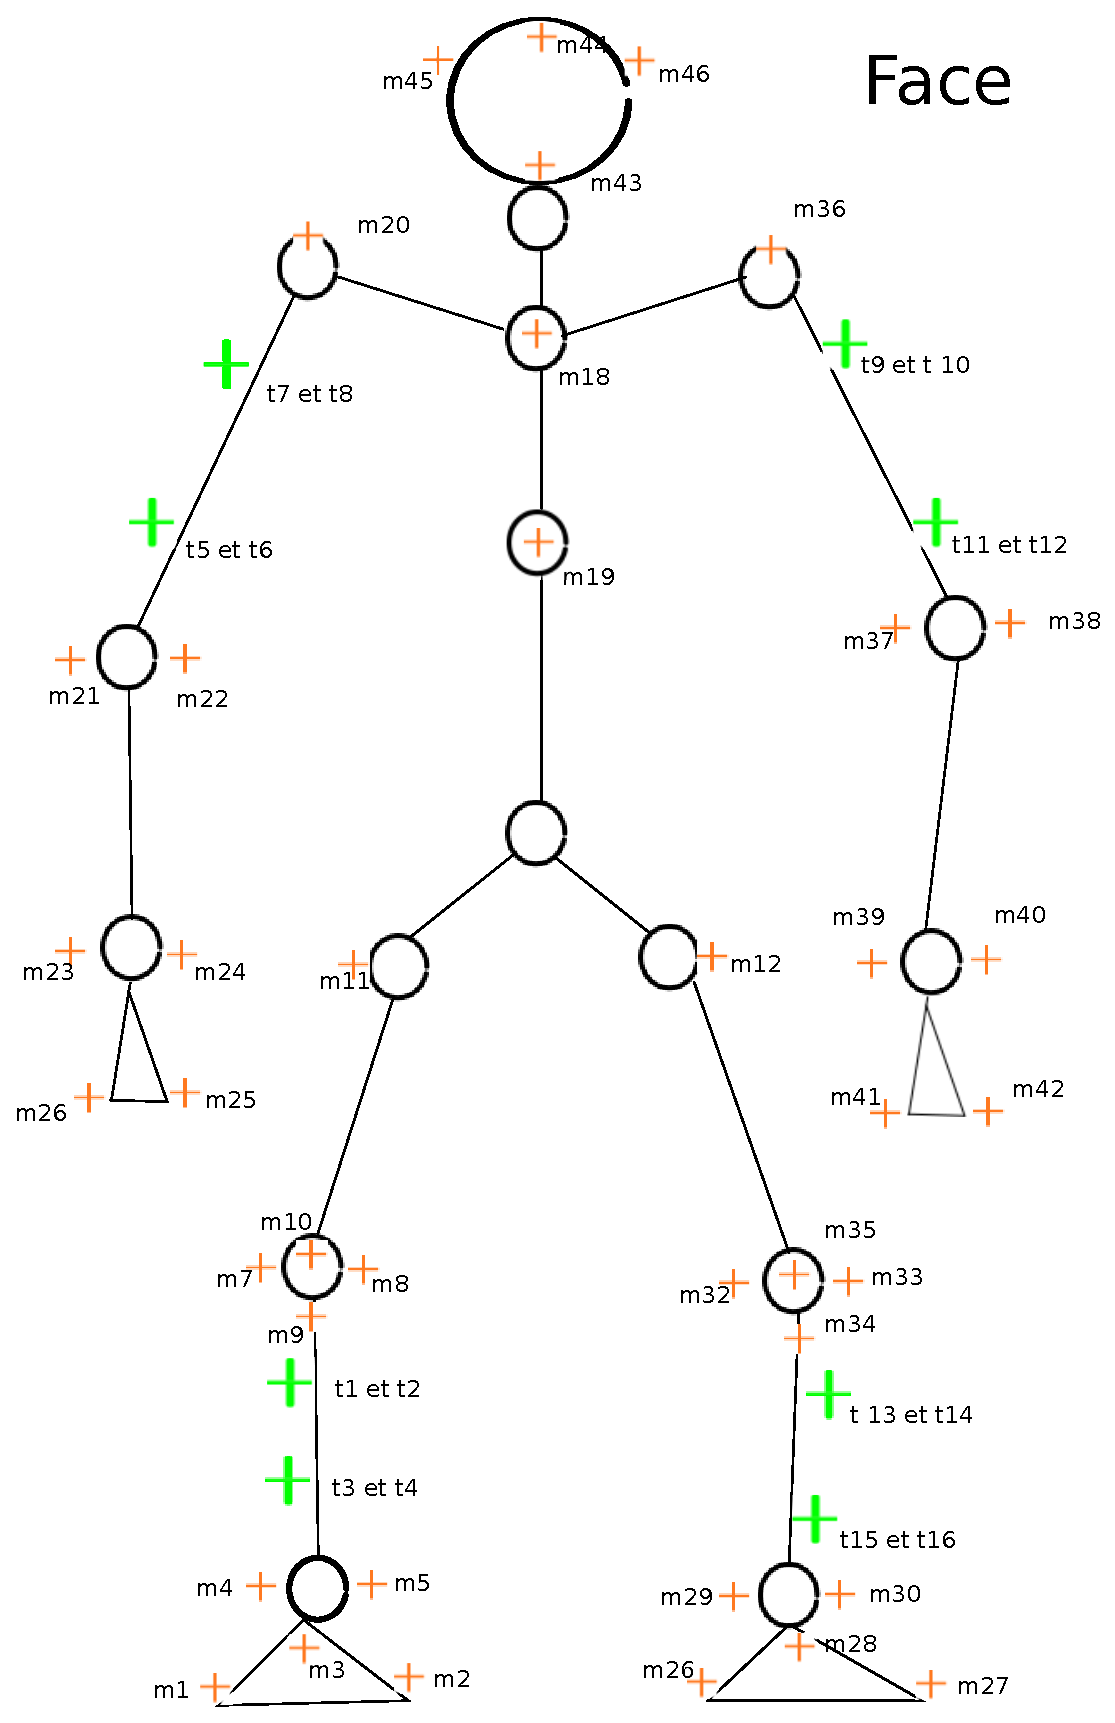
\includegraphics[width=0.7\columnwidth]{images/modeleHomme.eps}
\label{fig:marqueursFace}
\caption{Vue de face : positionnement des marqueurs. En orange, les marqueurs biomécaniques et en vert des marqueurs techniques.}
\end{figure}

\begin{figure}
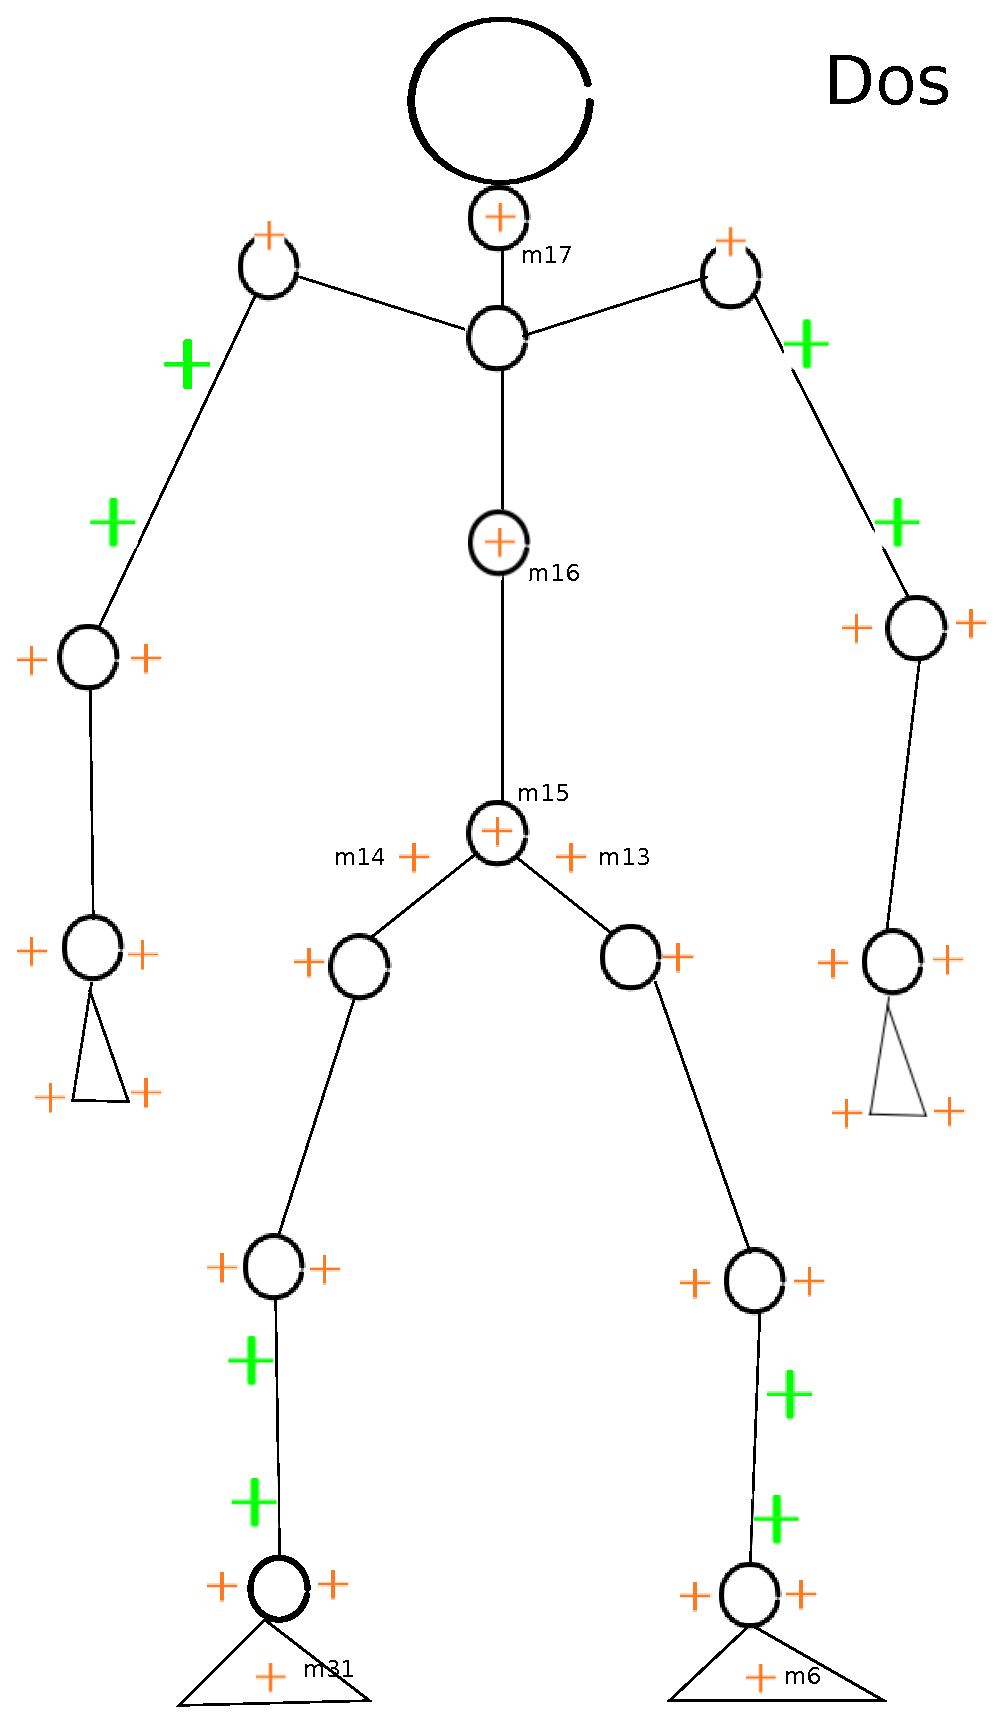
\includegraphics[width=0.7\columnwidth]{images/modeleHommeDos.eps}
\label{fig:marqueursDos}
\caption{Vue de dos : positionnement des marqueurs. En orange, les marqueurs biomécaniques et en vert des marqueurs techniques.}
\end{figure}

\begin{figure}
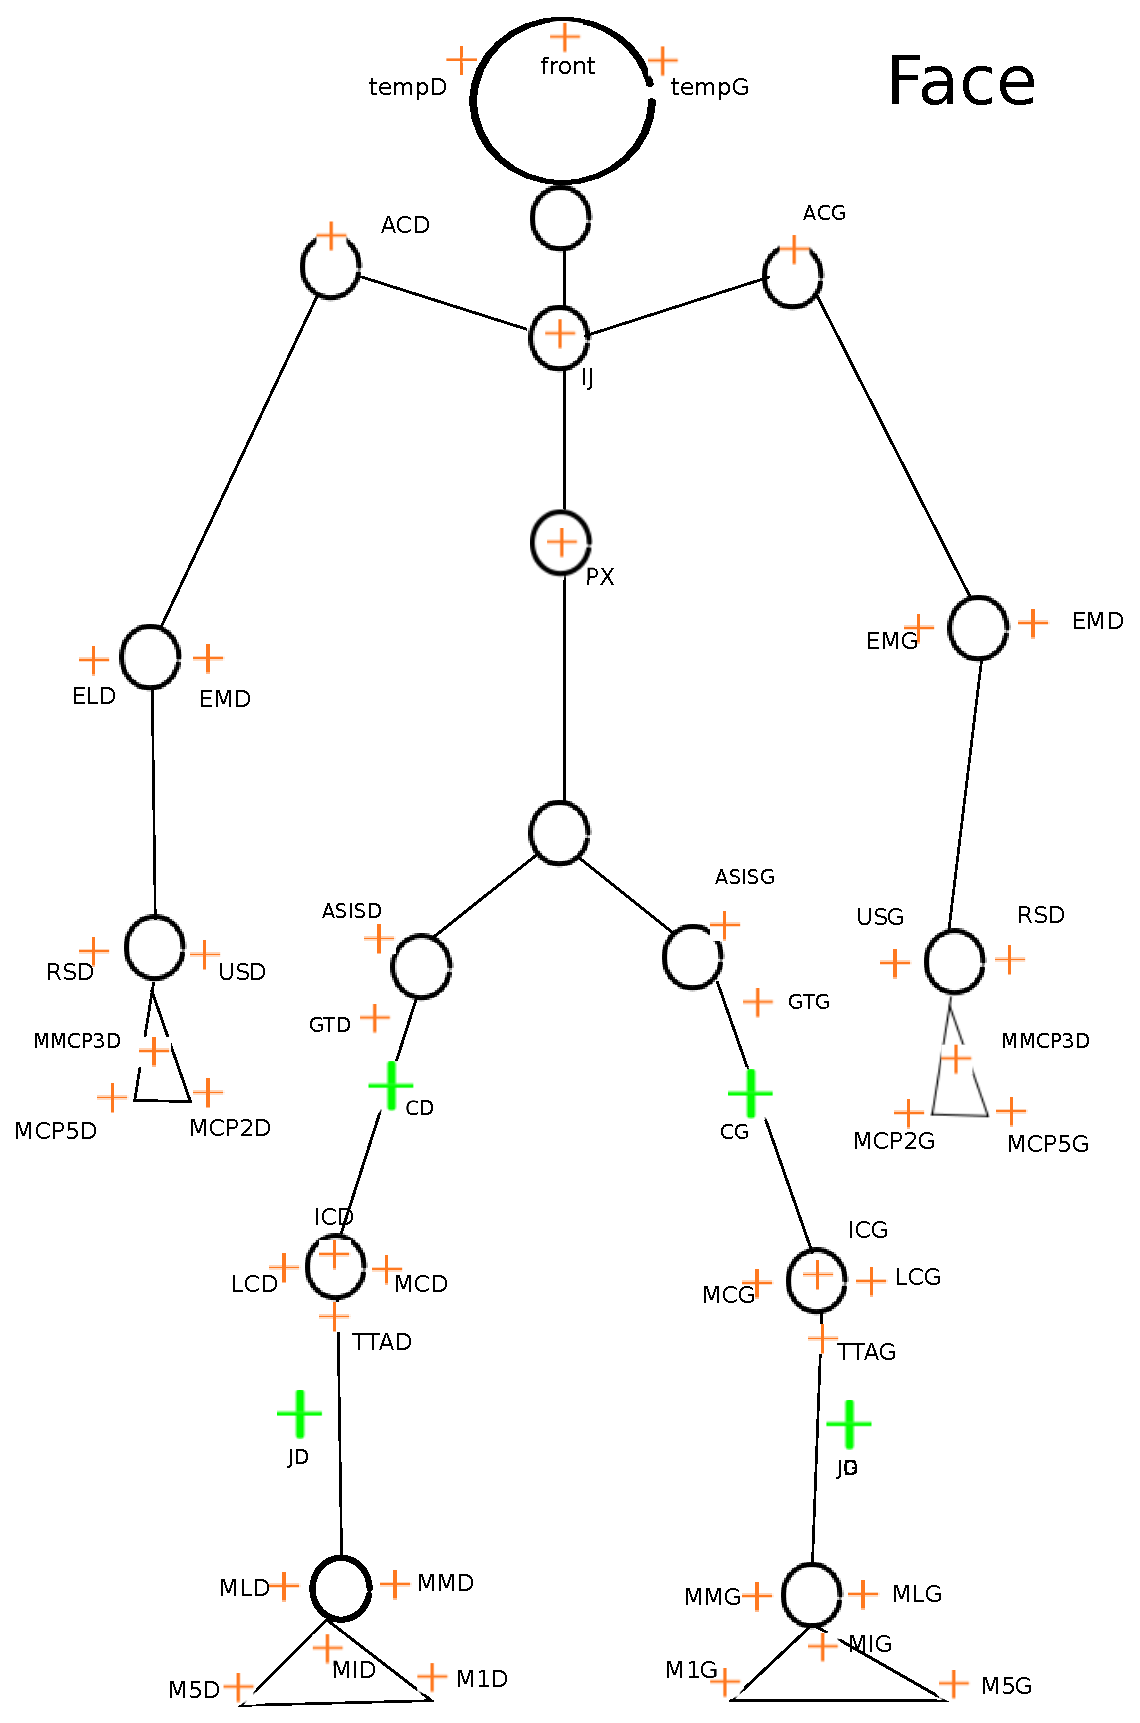
\includegraphics[width=0.7\columnwidth]{images/modeleHommeQualisys.eps}
\label{fig:marqueursFace}
\caption{Vue de face : Nomenclature modele qualisys}
\end{figure}

\begin{figure}
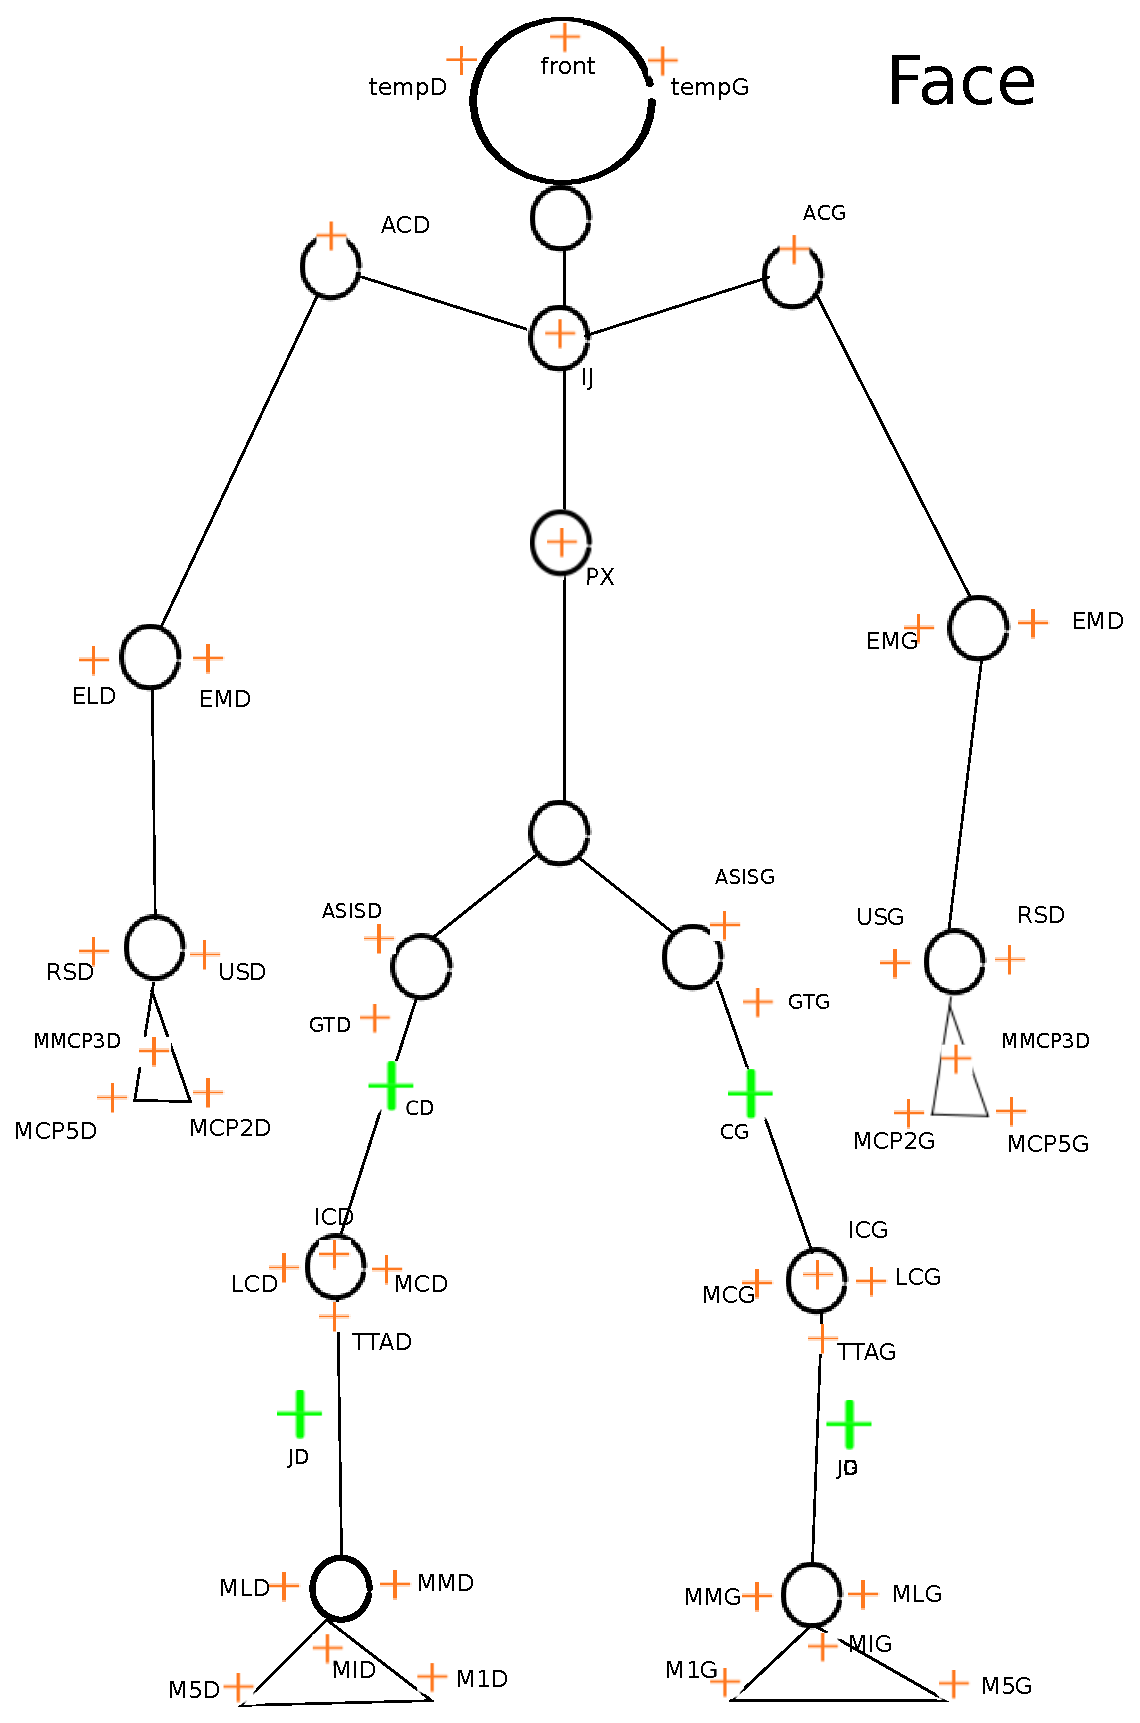
\includegraphics[width=0.7\columnwidth]{images/modeleHommeQualisys.eps}
\label{fig:marqueursDos}
\caption{Vue de dos : Nomenclature modele qualisys}
\end{figure}


\begin{itemize}
\item Pied droit
\begin{itemize}
\item $m1$ et $m2$ (ajout) sur les phalanges métatarses mediales et latérales
\item $m3$ sur l'articulation du 3e métatarse (IM)
\item $m4$ et $m5$ respectivement sur le maleole latérale (LM) et médiale (MM)
\item $m6$ (ajout) sur le talon
\end{itemize}
\item Genou droit
\begin{itemize}
\item $m7$ (LC) la limite externe condyle tibial lateral
\item $m8$ (MC) la limite interne du condyle tibial médial
\item $m9$ (TT) sur la tuberosité tibiale
\item $m10$ (IC) a mi distance de $m7$ et $m8$
\end{itemize}
\item Hanches
\begin{itemize}
\item$m11$ et $m12$  (ASIS)  sur les parties antérieures supérieures des os iliaques droit et gauche
\item $m13$ et $m14$ (PSIS)  sur les parties postérieures supérieures des os iliaques droit et gauche
\item  $m15$ (mid PSISs) a mi distance de $m12$ et $m14$
\end{itemize}
\item Torse
\begin{itemize}
\item $m16$ (T8) sur la 8e vertebre thoracique
\item $m17$ (C7) sur la 7e cervicale
\item $m18$ (IJ) au niveau de la fourchette sternale supérieure
\item $m19$ (PX) au niveau du processus xiphoïde
\end{itemize}
\item Epaule droite
\begin{itemize}
\item $m20$ (AC) au niveau de l'articulation acromio-claviculaire
\end{itemize}
\item{Coude droit}
\begin{itemize}
\item $m21$ (EL) Epicondyle latérale de l'humérus
\item $m22$ (EM) Epicondyle médiale de l'humérus
\end{itemize}
\item{Poignet droit}
\begin{itemize}
\item $m23$ (RS) styloïde radiale
\item $m24$ (US) styloïde cubitale
\end{itemize}
\item{Main droite}
\begin{itemize}
\item $m25$ (ajout) à l'exterieur de la 1e articulation métacarpo phalangienne
\item $m26$ (ajout) à l'exterieur de la 5e  articulation métacarpo phalangienne
\end{itemize}
\item {Côté gauche du corps} : $m27-m42$ construit par symétrie par rapport au côté droit.
\item {Tête}
\begin{itemize}
\item $m44$ (Front) front
\item $m45$ (tempD) et $m46$ (tempG) tempes droites et gauches
\end{itemize}

\end{itemize}

Remarques :

\begin{itemize}
\item Lorsque les marqueurs ne sont pas mentionnés dans le document de référence \cite{Wu02, Wu05}, j'ai noté "ajout".
\item J'ai ajouté un marqueur sur le talon et deux marqueurs sur les phalanges métatarses 1 et 6  pour mieux capturer le mouvement du pied
\item Je n'ai pas mis le marqueur SC sur l'articulation sterno-claviculaire pour ne pas la confondre avec le marqueur IJ de la fourchette sternale supérieure. Pensez vous qu'il faut la rajouter ?
\item Je n'ai pas les points sur la scapula (omoplate), je ne pense pas que cela soit nécessaire pour notre mouvement
\end{itemize}

\subsubsection{Positionnement des marqueurs sur le déambulateur }

La figure \ref{fig:deambulateur} présente le positionnement des marqueurs sur le déambulateur. 

\begin{itemize}
\item $d1$ et $d5$ sont placés sur les poignée droite et gauche, sur la partie tenant le frein
\item $d2$ et $d6$ sont situé au niveau de l'intersection des deux montants
\item $d9$ est situé entre $d2$ et $d6$ 
\item $d3$ et $d7$ sont placés sur les bouchons en plastique couvrant l'axe vertical des roues avant (les roues avant étant des roues folles, on ne met rien sur leur axe de rotation horizontal)
\item $d4$ et $d8$ sont placés sur l'axe de rotation des roues arrières.

\end{itemize}

\begin{figure}
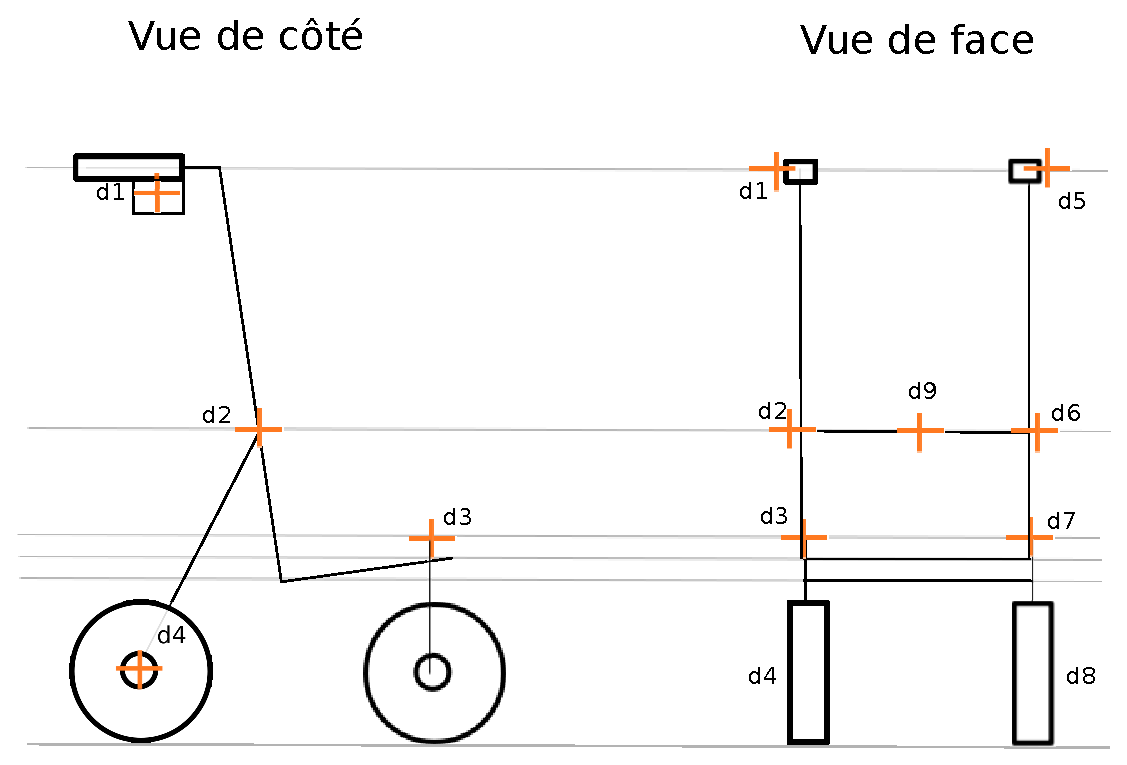
\includegraphics[width=0.7\columnwidth]{images/deambulateur.eps}
\label{fig:deambulateur}
\caption{Vue de face et vue de côté, positionnement des marqueurs sur le déambulateur.}
\end{figure}


\subsection{Equipement du déambulateur}

\subsubsection{Encodeurs}

Le déambulateur est équipé d'un encodeur sur chaque roue.
La figure \ref{fig:encodeur} présente le montage de cette encodeur. On essaye de faire des montages en pince au maximum pour éviter de modifier la structure du déambulateur.

\begin{figure}
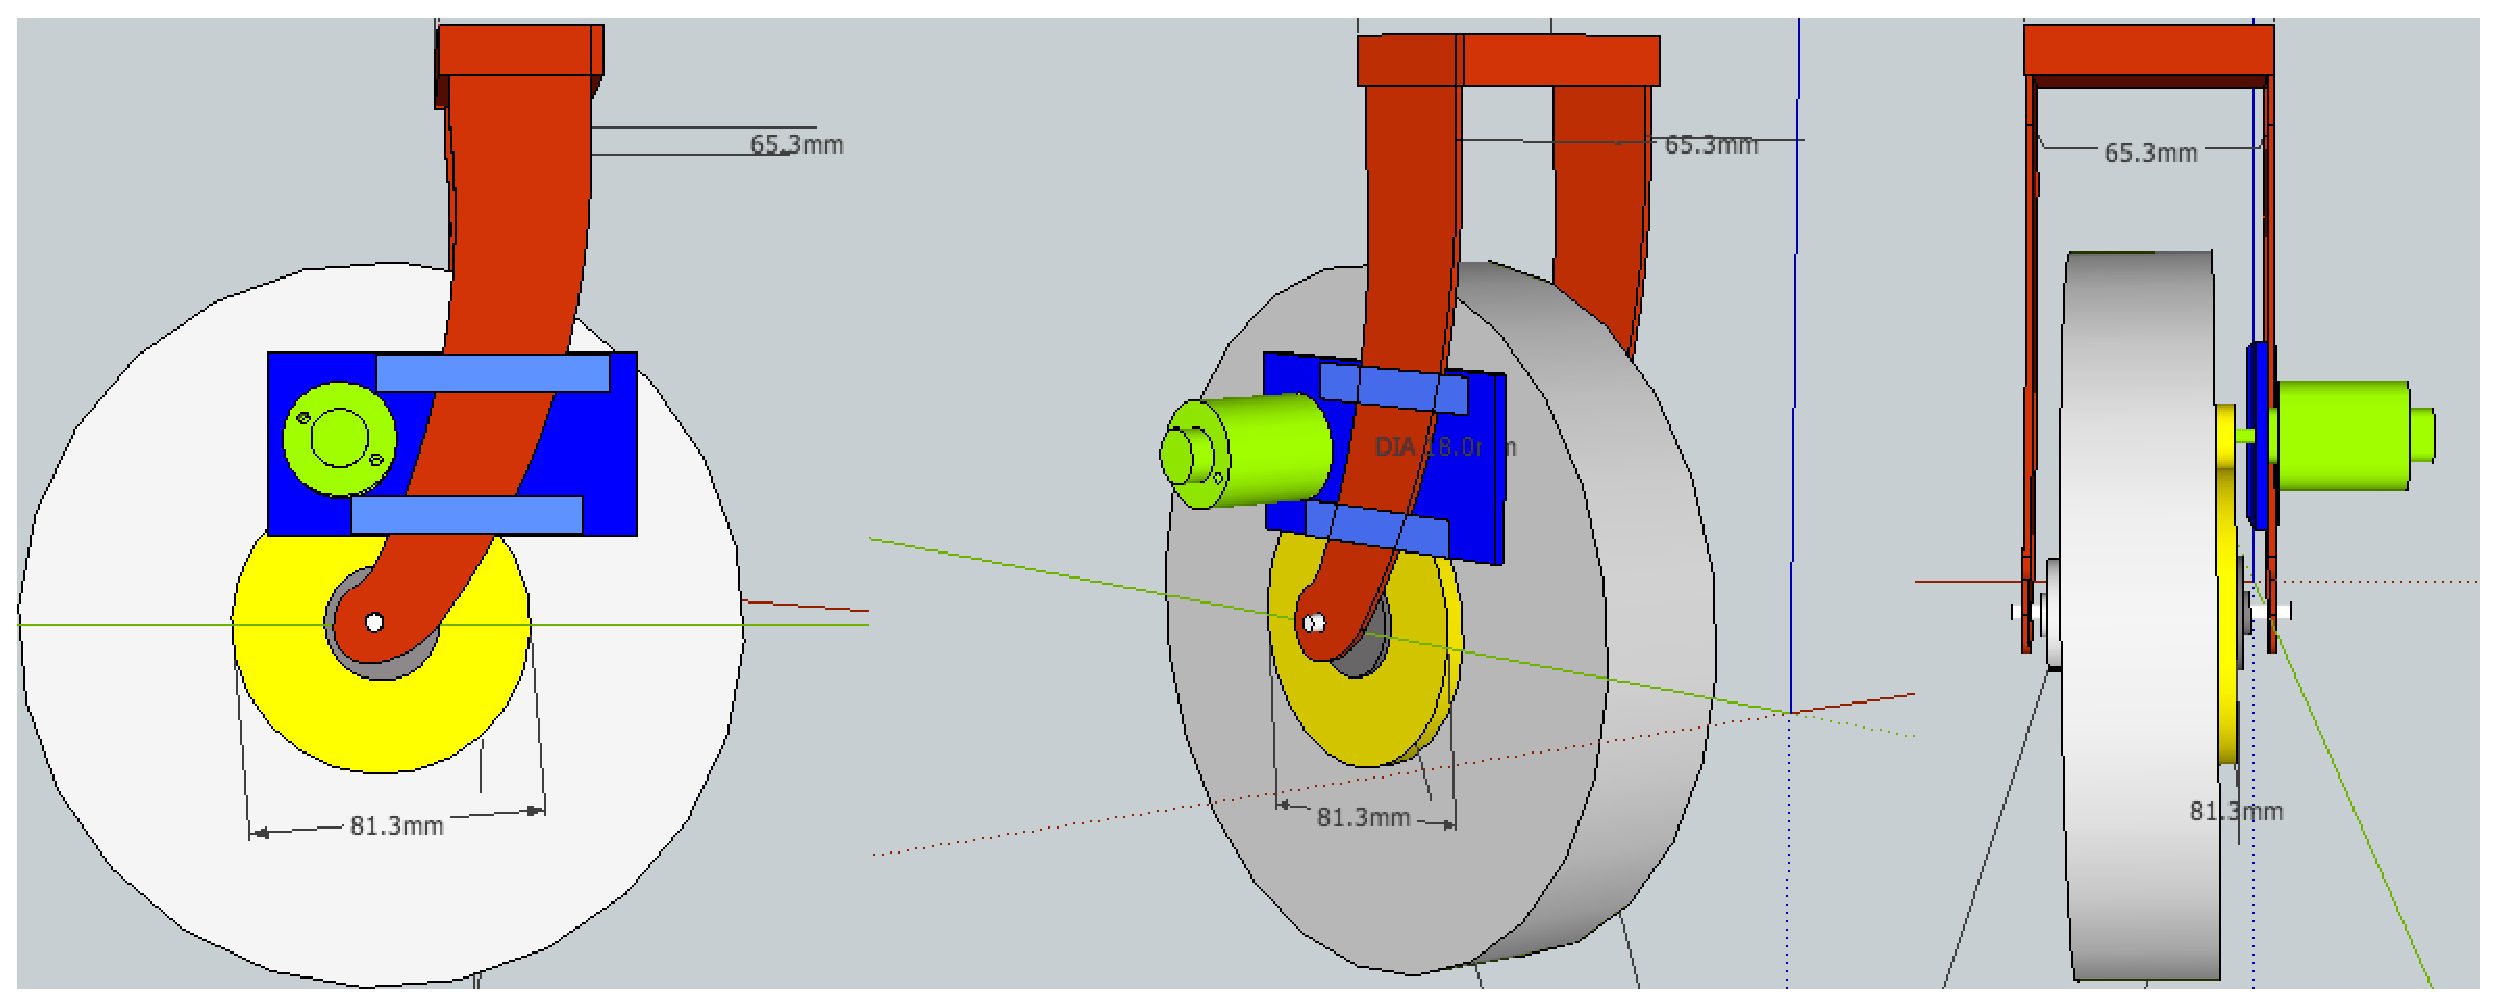
\includegraphics[width=0.8\columnwidth]{images/encodeur.eps}
\label{fig:encodeur}
\caption{Montage des encodeurs sur les roues.}
\end{figure}

\subsubsection{Gyro, accelero}

Le déambulateur est équipé d'une central inertielle avec gyro, accéléromètre et magneto.

\subsubsection{Kinect}

Une kinect est fixée sur le déambulateur pour capter la posture du sujet. Dans un premier temps, uniquement la position des pieds.

\subsubsection{Banc de stéréovision}

En plus/a la place de la kinect, un banc de stéréovision peut être monté sur le déambulateur.
Pour l'instant, le banc de stéréovision n'est pas monté.

\section{Déroulement de la manip}

\subsection{Synchronisation des horloges des ordinateurs}
\subsubsection{Principe général}
Durant les expérimentations, trois ordinateurs interviennent de manière ``active''~:
\begin{enumerate}
	\item Une machine fixe fonctionnant sous Windows XP permettant d'enregistrer les données issues du Qualisys,
	\item Un ordinateur portable tournant sous Linux Ubuntu fourni par INRIA dédié au traitement des données Kinect et banc stéréo (traitement du banc stéré à venir),
	\item Le mini-ordinateur Phidget SBC tournant sous une version allégée de Linux Debian dédié au traitement des autres capteurs.
\end{enumerate}
Chacun des programmes d'acquisition date les données obtenues en fonction de l'\textbf{horloge interne} fournie par l'ordinateur sur lequel est branché le capteur. Pour garantir un rejeu cohérent des données, il est nécessaire que les horloges des différents ordinateurs soient synchronisées. Pour cela, les 3 ordinateurs sont mis en réseau à l'aide d'une borne wifi et le protocole NTP (Network Time Protocl) est utilisé pour synchroniser les horloges~:
\begin{enumerate}
	\item La borne wifi génère un réseau wifi ouvert avec serveur DHCP (attribution automatique d'IP) et possède un port ethernet filaire.
	\item Le PC portable INRIA est connecté sur le réseau Wifi. Le serveur NTP est lancé.
	\item La station fixe étant dépourvue de carte wifi, il a été choisi de la relier à la borne à l'aide du réseau filaire ethernet (plusieurs cartes réseaux sont présentes sur cette machine~; cela ne perturbe donc pas l'utilisation des caméras du Qualisys qui sont également branchées en ethernet sur une autre interface). Un client NTP est lancé sur cette machine.
	\item Le mini-PC se connecte automatiquement à la borne wifi au démarrage si elle est détectée. Un client ntp est lancé sur cette machine.
\end{enumerate} 

\subsubsection{Mise en route du serveur et des clients NTP}
\begin{enumerate}
	\item Une fois toutes les machines connectées, lancer d'abord le serveur ntp sur le PC portable~:\emph{sudo service ntp start} (ou \emph{restart} en cas de changement du fichier de conf ntp)
	\item Sur le mini-PC, éditer le fichier \emph{/etc/ntp.conf} après s'être connecté dessus avec une connexion ssh. Editer la ligne \emph{server} et indiquer l'adresse IP du PC portable si ce n'est pas la bonne. (TODO~: voir si on ne peut pas utiliser un dns, quitte à supprimer le service DHCP de la borne wifi. Cela permettrait d'utiliser les noms de PC et de ne pas revérifier à chaque fois l'adresse IP).
	\item Un client ntp est déjà lancé par défaut sur le minipc. Dans un premier temps, on va l'arrêter~: \emph{service ntp stop}
	\item Lancer le client ntp de manière unique pour vérifier que la connexion s'établie correctement~: \emph{ntpd -q -g} (\emph{-q} sert à mettre à jour et quitter, \emph{-g} à forcer le client à se mettre à jour même si le décalage est très grand). Si tout se passe bien, une réponse doit apparaître indiquant l'offset appliqué.
	\item Relancer la commande de mise à jour unique \emph{ntpd -q} (\emph{-g} n'est plus utile normalement). On doit avoir un décalage de l'ordre du centième de seconde. 
	\item Lancer le service ntp afin de laisser le service effectuer les micro-ajustements nécessaires (\emph{service ntp start}). 
	\item Sur la station fixe, un script bash est présent sur le bureau (\emph{NTP.bat}). Editer le script et ajuster l'adresse IP du serveur si nécessaire. Modifier l'horloge Windows afin de se décaler franchement de l'heure du PC portable. Exécuter le script depuis un terminal et vérifier que le message (\emph{La commande s'est terminée correctement} apparaisse bien à la fin. L'heure dans la barre des tâches Windows doit se modifier. Eventuellement, relancer le script pour être certain de se synchroniser finement avec le PC portable (il est possible que la première synchro ne soit pas très fine si le décalage est trop important). 
\end{enumerate}

\subsection{Lancement des scripts}
Une fois la synchronisation des horloges effectuées, on peut lancer les expérimentations. Tout se réalise à distance via ssh (sauf pour le Qualisys dont l'acquisition se fait depuis la station de travail Windows).
\subsubsection{PC portable~: la Kinect}
L'acquisition de la Kinect se fait via ROS. Ainsi, avant d'acquérir les données, il faut lancer ROS ainsi que le driver Kinect.
\begin{enumerate}
	\item Dans un terminal, taper \emph{roscore} pour lancer un serveur ROS
	\item Dans un autre terminal, lancer un n{\oe}ud Kinect par la commande \linebreak \emph{rosrun openni{\_}camera openni{\_}node}.
\end{enumerate}
Dans la version actuelle du code d'acquisition, le n{\oe}ud ROS effectue un retour \linebreak graphique toutes les $step\_viewer$ images et sauvegarde une image sur $step\_HW$. Ces valeurs doivent être ajustées dans le code \emph{kinectListener.cpp} (TODO~: faire en sorte de les passer en paramètres pour ne pas avoir à recompiler). Pour cela~:
\begin{enumerate}
	\item Editer le fichier à l'aide de la commande \emph{rosed kinectGrabber kinectListener.cpp}.
	\item Compiler le code à l'aide de la commande \emph{rosmake kinectGrabber}.
\end{enumerate}
On a alors trois cas~:
\begin{enumerate}
	\item On veut lancer le code pour voir en live le rendu (ex. positionner la caméra). Dans ce cas, il vaut mieux ne pas sauvegarder les images. On mettra alors $step\_viewer$ à 1 et une grande valeur pour $step\_HW$.
	\item On veut lancer le code pour avoir tout sauvegarder tout en ayant un retour caméra. Ceci n'est possible que si on visualise directement sur le PC. Dans ce cas, il choisir $step\_viewer>10$ pour éviter que la sauvegarde d'images ne prenne du retard.
	\item On veut lancer le code pour tout sauvegarder mais à distance. Pour cela, il ne faut pratiquement faire aucune mise à jour de l'image de contrôle car l'export du flux pourrait provoquer des ralentissement. On prendra alors $step\_viewer$ très grand. 
\end{enumerate}
\textbf{Attention~:} lors de l'utilisation de la Kinect à distance, il est nécessaire de se connecter grâce à \emph{ssh -X}. Même si on n'affiche pratiquement rien dans le retour vidéo, l'affichage de la fenêtre indique que la capture a bien commencée.

Finalement, le lancement du script se fait par \emph{rosrun KinectGrabber KinectListener pathToSave}. Le paramètre \emph{pathToSave} indique le lieu où doivent être sauvegardées les données. S'il n'existe pas, il sera créer. \textbf{S'il existe, il sera effacé. Faire attention à ne pas appeler deux fois de suite la commande avec la même valeur de répertoire sans avoir sauvegarder les données au préalable}. Le dossier contiendra alors 3 sous-dossiers~:
\begin{enumerate}
	\item \emph{depth\_image} contient l'ensemble des images tiff représentant des cartes de profondeurs. Ces cartes sont pré-traitées par le driver et ramenées directement dans le repère caméra.  
	\item \emph{RGB\_image} contient l'ensemble des images RGB.
	\item \emph{TS} contient deux fichiers de \emph{timestamps} (un pour les images RGB et un pour les cartes de profondeurs). La première colonne correspond au numéro de l'image (en référence aux noms de fichiers) et l'autre au temps PC depuis la date ``epoch''.
\end{enumerate}
\subsubsection{SBC~: la centrale inertielle et les encodeurs}
Pour acquérir des données sur le SBC, il faut impérativement se connecter dessus en ssh puis se rendre dans le répertoire \emph{/root/handiwalker}. De là, le binaire \emph{bin/spatial} permet d'effectuer l'acquisition de la centrale inertielle et le binaire \emph{bin/encoder} permet d'effectuer l'acquisition des encodeurs. Le programme d'acquisition de la centrale inertielle (resp. encodeurs) enregistre les données dans le fichier \emph{dataSaved/spatial} (resp. \emph{dataSaved/encoder}).

\textbf{Attention~:} A chaque lancement des binaires exécutables, les fichiers de sauvegarde sont écrasés. Il faut donc bien penser à faire une sauvegarde du fichier acquis.

\noindent Les données de la centrale inertielle sont réparties en 10 colonnes~:
\begin{enumerate}
	\item Temps en seconde depuis la date ``epoch''
	\item Accélération suivant l'axe $x$ (en $\mathrm{g}$)
	\item Accélération suivant l'axe $y$ (en $\mathrm{g}$)
	\item Accélération suivant l'axe $z$ (en $\mathrm{g}$)
	\item Vitesse de rotation suivant l'axe $x$ (en $\deg.\mathrm{s}^{-1}$)
	\item Vitesse de rotation suivant l'axe $y$ (en $\deg.\mathrm{s}^{-1}$)
	\item Vitesse de rotation suivant l'axe $z$ (en $\deg.\mathrm{s}^{-1}$)
	\item Champ magnétique suivant l'axe $x$ (unité ?)
	\item Champ magnétique suivant l'axe $y$ (unité ?)
	\item Champ magnétique suivant l'axe $z$ (unité ?)
\end{enumerate}

\noindent Les données des encodeurs sont quant à elles réparties en colonnes~:
\begin{enumerate}
	\item Numéro du codeur (0 pour la roue gauche, 1 pour la roue droite)
	\item Position absolue (en terme de nombre d'impulsions depuis le début de la manipulation)
	\item Position relative (nombre d'impulsions depuis la dernière info donnée par le codeur concerné)
	\item Distance parcourue par la roue concernée depuis le début de la manipulation
	\item Distance parcourue par la roue concernée depuis SA dernière acquisition (ne prend pas en compte l'autre roue)
	\item Temps écoulé depuis la dernière acquisition du codeur en microsecondes (non utilisé, on ne connaît pas la référence initiale~; par ailleurs, la mesure avec un \emph{gettimeofday} du SBC ne pose pas de problème de dérive (éventuellement un très léger offset)
	\item Temps mesuré par le SBC depuis la date ``epoch''
\end{enumerate}

\subsection{Sauvegarde et stockage des données}

TODO : Scripts, nomenclature et lieu de stockage ...


\bibliographystyle{plain} 
\bibliography{biblio}


\end{document}
